\chapter{Experimental Results}
\label{chap:experimental-results}

\section{Overview of the Statistical Output}
\label{sec:results-statistical-output-overview}

This chapter reports the results of the statistical analysis applied to the
graph-theoretical EEG connectivity features. The aim was to evaluate whether
network properties differed across the temporal windows Baseline, T0, T1, and
T2, and whether any observed effects were consistent across seizure-level and
subject-average analyses.

The final statistical input contained \num{11376} graph-level observations.
Eight graph metrics were analyzed, producing \num{91008} long-format rows. The
dataset included \num{24} subject/case identifiers and \num{159} usable
seizures. Of these, \num{155} seizures had complete values across all four
windows and were included in Baseline-inclusive seizure-level omnibus testing.
All \num{159} seizures had complete values across the three preictal windows
T0, T1, and T2 and were therefore available for the preictal trend analysis.

The analysis was performed separately for each combination of graph metric,
connectivity method, and frequency band. Since \num{8} graph metrics,
\num{3} connectivity methods, and \num{6} frequency bands were analyzed, the
full seizure-level analysis included \num{144} metric--method--band
combinations. This produced \num{144} omnibus window-effect tests, \num{432}
planned Baseline-vs-preictal post-hoc contrasts, and \num{144} preictal trend
tests.

The subject-average sensitivity analysis produced \num{13824} subject-average
rows. In this analysis, each subject/case identifier contributed one average
trajectory for each metric, method, band, and window combination. The
subject-average analysis produced \num{112} omnibus tests with valid model
output and \num{432} planned post-hoc contrasts.

After Benjamini--Hochberg FDR correction, the main finding was a temporal-window
effect for global efficiency computed from delta-band coherence networks. This
effect was present in both the seizure-level omnibus analysis and the
subject-average omnibus analysis. At the seizure level, the corresponding
post-hoc analysis localized the strongest difference to the Baseline-vs-T1
contrast. No preictal trend test survived FDR correction, and no
subject-average post-hoc contrast survived FDR correction.

\begin{table}[H]
    \centering
    \begin{tabular}{p{0.32\textwidth}p{0.58\textwidth}}
        \toprule
        Analysis family & FDR-significant result \\
        \midrule
        Seizure-level omnibus tests
        & Global efficiency, coherence, delta band \\

        Seizure-level post-hoc contrasts
        & Global efficiency, coherence, delta band, Baseline vs T1 \\

        Seizure-level preictal trend tests
        & No FDR-significant trend effects \\

        Subject-average omnibus tests
        & Global efficiency, coherence, delta band \\

        Subject-average post-hoc contrasts
        & No FDR-significant post-hoc contrasts \\
        \bottomrule
    \end{tabular}
    \caption{Summary of FDR-significant findings across the main statistical
    output families.}
    \label{tab:results-significant-output-summary}
\end{table}

Overall, the results indicate that the most robust statistical effect in the
full dataset was an increase in delta-band coherence global efficiency during
the preictal period, especially in the T1 window. The following sections report
the seizure-level omnibus tests, post-hoc contrasts, preictal trend results,
and subject-average sensitivity analysis in more detail.

\section{Seizure-Level Omnibus Window Effects}
\label{sec:results-seizure-level-omnibus}

The seizure-level omnibus analysis tested whether each graph metric showed an
overall difference across Baseline, T0, T1, and T2. A separate test was
performed for each metric--method--band combination, resulting in \num{144}
omnibus window-effect tests.

After Benjamini--Hochberg FDR correction, one seizure-level omnibus effect
remained statistically significant. This effect was observed for global
efficiency computed from delta-band coherence networks. The test included
\num{155} complete seizures from \num{24} subject/case identifiers and showed a
significant effect of temporal window
($\chi^2(3) = 21.11$, $p_{\mathrm{uncorrected}} = 0.000100$,
$p_{\mathrm{FDR}} = 0.014367$).

\begin{table}[H]
    \centering
    \begin{tabular}{llllrrrr}
        \toprule
        Metric & Method & Band & Test & $n$ & $\chi^2$ & $p$ & $p_{\mathrm{FDR}}$ \\
        \midrule
        Global efficiency
        & Coherence
        & Delta
        & Window effect
        & 155
        & 21.11
        & 0.000100
        & 0.014367 \\
        \bottomrule
    \end{tabular}
    \caption{FDR-significant seizure-level omnibus window effect.}
    \label{tab:seizure-level-significant-omnibus}
\end{table}

The descriptive means for this metric showed an increase from Baseline to the
preictal windows. Mean delta-band coherence global efficiency was
\num{0.224424} at Baseline, \num{0.228493} at T0, \num{0.234382} at T1, and
\num{0.233047} at T2. The highest mean value was therefore observed in T1,
followed by a small decrease in T2.

\begin{table}[H]
    \centering
    \begin{tabular}{lrrrr}
        \toprule
        Window & $n$ & Mean & SD & 95\% CI \\
        \midrule
        Baseline & 155 & 0.224424 & 0.036161 & [0.218687, 0.230162] \\
        T0       & 159 & 0.228493 & 0.036656 & [0.222751, 0.234234] \\
        T1       & 159 & 0.234382 & 0.033300 & [0.229166, 0.239598] \\
        T2       & 159 & 0.233047 & 0.033635 & [0.227779, 0.238316] \\
        \bottomrule
    \end{tabular}
    \caption{Descriptive statistics for seizure-level delta-band coherence
    global efficiency across temporal windows.}
    \label{tab:seizure-level-global-efficiency-delta-coherence-descriptives}
\end{table}

No other seizure-level omnibus test survived FDR correction. Therefore, the
only robust seizure-level evidence for a temporal-window effect was found for
global efficiency in delta-band coherence networks. The corresponding planned
post-hoc comparisons are reported in the next section.

\section{Post-hoc Baseline-vs-Preictal Comparisons}
\label{sec:results-posthoc-baseline-preictal}

Planned post-hoc comparisons were used to determine which preictal windows
differed from Baseline. These comparisons were interpreted primarily for
metric--method--band combinations that showed a significant omnibus
window-effect after FDR correction.

Only one post-hoc contrast survived FDR correction. This was the
Baseline-vs-T1 comparison for global efficiency in delta-band coherence
networks. The paired comparison included \num{155} seizures from \num{24}
subject/case identifiers. Mean global efficiency increased from
\num{0.224424} at Baseline to \num{0.233575} at T1, corresponding to a mean
paired difference of \num{0.009150}. This contrast was significant after FDR
correction ($t(154) = 4.22$, $p_{\mathrm{uncorrected}} = 0.000042$,
$p_{\mathrm{FDR}} = 0.018111$, Cohen's $d_z = 0.339$).

\begin{table}[H]
    \centering
    \begin{tabular}{lrrrrrr}
        \toprule
        Contrast & Baseline mean & Preictal mean & Difference
        & $t$ & $p$ & $p_{\mathrm{FDR}}$ \\
        \midrule
        Baseline vs T0
        & 0.224424 & 0.227550 & 0.003126
        & 1.35 & 0.177660 & 0.600708 \\

        Baseline vs T1
        & 0.224424 & 0.233575 & 0.009150
        & 4.22 & 0.000042 & 0.018111 \\

        Baseline vs T2
        & 0.224424 & 0.231975 & 0.007551
        & 3.08 & 0.002427 & 0.288818 \\
        \bottomrule
    \end{tabular}
    \caption{Seizure-level post-hoc comparisons for delta-band coherence
    global efficiency.}
    \label{tab:posthoc-global-efficiency-delta-coherence}
\end{table}

The Baseline-vs-T0 comparison was not significant, indicating that the earliest
preictal window did not differ clearly from Baseline for this metric. The
Baseline-vs-T2 comparison showed an uncorrected difference, but it did not
survive FDR correction. Therefore, the only statistically robust localized
post-hoc effect was the increase from Baseline to T1.

The Wilcoxon signed-rank sensitivity analysis showed the same direction of
change for the Baseline-vs-T1 contrast, but its FDR-corrected value was just
above the significance threshold
($p_{\mathrm{uncorrected}} = 0.000121$,
$p_{\mathrm{FDR}} = 0.052186$). Thus, the post-hoc evidence was strongest in
the paired $t$-test, while the non-parametric sensitivity result supported the
same direction but did not meet the corrected threshold.

No other Baseline-vs-preictal contrast survived FDR correction. Therefore, the
post-hoc analysis localized the main seizure-level omnibus effect to a
Baseline-to-T1 increase in delta-band coherence global efficiency.

\section{Preictal Trend Analysis}
\label{sec:results-preictal-trend}

The preictal trend analysis tested whether graph metrics changed linearly across
T0, T1, and T2 as seizure onset approached. Unlike the Baseline-vs-preictal
comparisons, this analysis did not include the Baseline window. It focused only
on directional change within the preictal period.

A total of \num{144} seizure-level trend tests were performed, one for each
metric--method--band combination. All \num{159} usable seizures contributed to
the trend analysis because complete T0, T1, and T2 values were available for all
seizures.

No preictal trend survived Benjamini--Hochberg FDR correction. Therefore, the
analysis did not provide corrected evidence for a consistent monotonic increase
or decrease across T0, T1, and T2 for any graph metric, connectivity method, or
frequency band.

For the main omnibus finding, delta-band coherence global efficiency showed a
positive preictal slope, indicating higher values closer to seizure onset.
However, this trend did not survive FDR correction
($\beta = 0.000759$ per minute, $p_{\mathrm{uncorrected}} = 0.030552$,
$p_{\mathrm{FDR}} = 0.347761$).

\begin{table}[H]
    \centering
    \begin{tabular}{lllrrrr}
        \toprule
        Metric & Method & Band & $n$ & Slope/min & $p$ & $p_{\mathrm{FDR}}$ \\
        \midrule
        Global efficiency
        & Coherence
        & Delta
        & 159
        & 0.000759
        & 0.030552
        & 0.347761 \\
        \bottomrule
    \end{tabular}
    \caption{Preictal trend result for the main significant omnibus metric.}
    \label{tab:preictal-trend-global-efficiency-delta-coherence}
\end{table}

These results suggest that the significant temporal-window effect observed for
delta-band coherence global efficiency was not explained by a strictly
monotonic T0--T2 trajectory. Instead, the main seizure-level effect was better
localized by the Baseline-vs-preictal post-hoc analysis, especially the
Baseline-vs-T1 comparison.

\section{Subject-Average Sensitivity Analysis}
\label{sec:results-subject-average-sensitivity}

The subject-average sensitivity analysis tested whether the main seizure-level
finding was also visible when each subject/case identifier contributed one
average trajectory. This analysis reduces the influence of subjects with many
seizures and provides a complementary subject-level view of the results.

The subject-average omnibus analysis identified one FDR-significant
temporal-window effect. As in the seizure-level analysis, this effect was found
for global efficiency computed from delta-band coherence networks. The model
included all \num{24} subject/case identifiers and showed a significant effect
of temporal window
($\chi^2(3) = 24.04$, $p_{\mathrm{uncorrected}} = 0.000025$,
$p_{\mathrm{FDR}} = 0.002748$).

\begin{table}[H]
    \centering
    \begin{tabular}{lllrrrr}
        \toprule
        Metric & Method & Band & $n$ & $\chi^2$ & $p$ & $p_{\mathrm{FDR}}$ \\
        \midrule
        Global efficiency
        & Coherence
        & Delta
        & 24
        & 24.04
        & 0.000025
        & 0.002748 \\
        \bottomrule
    \end{tabular}
    \caption{FDR-significant subject-average omnibus window effect.}
    \label{tab:subject-average-significant-omnibus}
\end{table}

The subject-average means followed the same general pattern as the
seizure-level analysis. Mean global efficiency was \num{0.222440} at Baseline,
\num{0.223423} at T0, \num{0.233735} at T1, and \num{0.229908} at T2. The
highest average value was again observed in T1.

\begin{figure}[H]
    \centering
    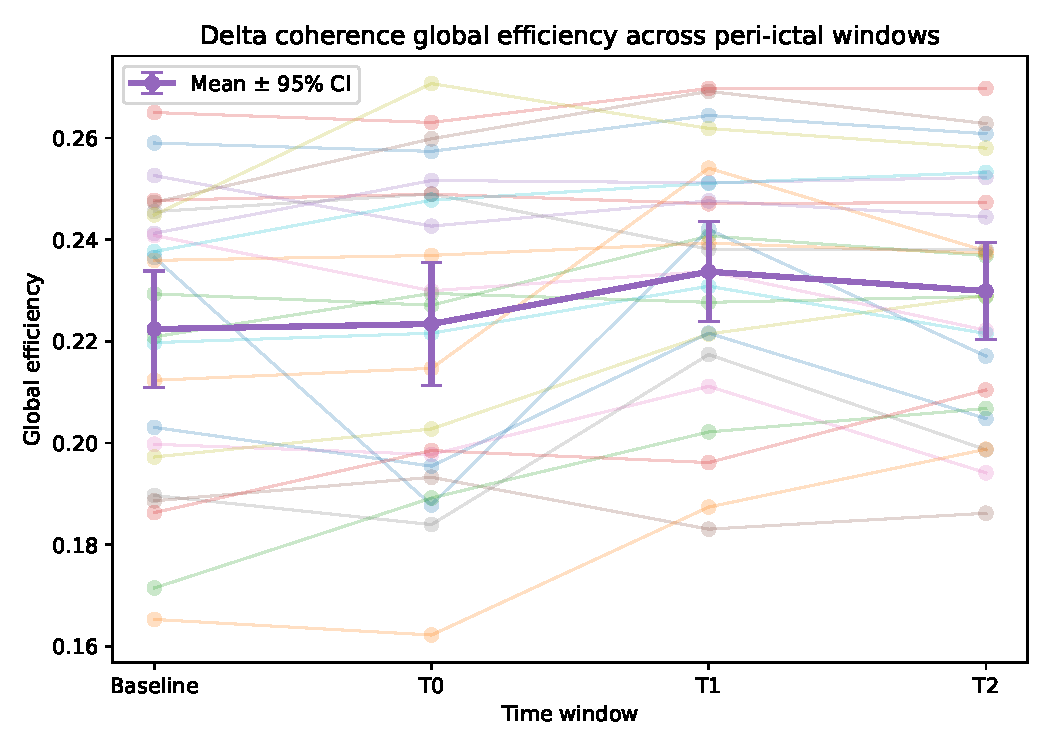
\includegraphics[width=0.85\textwidth]{figures/global_efficiency_coherence_delta_subject_average.pdf}
    \caption{Subject-average trajectory of delta-band coherence global
    efficiency across Baseline, T0, T1, and T2. Each subject/case identifier
    contributes one averaged value per temporal window.}
    \label{fig:global-efficiency-coherence-delta-subject-average}
\end{figure}

As shown in \cref{fig:global-efficiency-coherence-delta-subject-average}, the
subject-average trajectory increased from Baseline toward the preictal windows,
with the highest mean value in T1. This supports the seizure-level omnibus
finding by showing that the same pattern was present after averaging across
seizures within each subject/case identifier.

However, none of the subject-average Baseline-vs-preictal post-hoc contrasts
survived FDR correction. The Baseline-vs-T1 contrast showed the strongest
uncorrected effect
($t(23) = 4.40$, $p_{\mathrm{uncorrected}} = 0.000206$,
$p_{\mathrm{FDR}} = 0.089102$, Cohen's $d_z = 0.899$), but it did not meet the
corrected significance threshold. Therefore, the subject-average analysis
confirmed the overall temporal-window effect but did not localize a specific
Baseline-vs-preictal contrast after correction.

No other subject-average omnibus test survived FDR correction. Thus, the
subject-average analysis supported the main result observed at the seizure
level: delta-band coherence global efficiency was the only graph feature that
showed a robust temporal-window effect across both analysis levels.

\section{Summary of Main Findings}
\label{sec:results-summary-main-findings}

The full-dataset statistical analysis identified one robust graph-theoretical
effect after FDR correction. Global efficiency computed from delta-band
coherence networks showed a significant temporal-window effect in both the
seizure-level and subject-average omnibus analyses.

At the seizure level, the effect was localized by the planned post-hoc
comparisons to an increase from Baseline to T1. Mean global efficiency increased
from \num{0.224424} at Baseline to \num{0.233575} at T1, and this contrast
remained significant after FDR correction. The Baseline-vs-T2 comparison showed
the same direction of change but did not survive correction.

The preictal trend analysis did not identify any FDR-significant monotonic
T0--T1--T2 changes. Therefore, the main result should not be interpreted as a
strict linear increase toward seizure onset. Instead, the strongest evidence was
for a window-specific increase in delta-band coherence global efficiency,
especially around the T1 interval.

The subject-average sensitivity analysis supported the main finding at the
level of subject/case identifiers. The same metric--method--band combination
showed a significant omnibus window effect after averaging seizures within each
subject/case identifier. However, subject-average post-hoc contrasts did not
survive FDR correction, indicating that the localized Baseline-vs-T1 effect was
stronger at the seizure level than at the subject-average level.

No other graph metric, connectivity method, or frequency band combination
survived FDR correction in the omnibus, post-hoc, or trend analyses. Overall,
the results suggest that the most consistent preictal network alteration in this
dataset was a change in global integration of delta-band coherence networks,
rather than a broad effect across all graph metrics or all frequency bands.